\documentclass[xetex,12pt,compress,hyperref={xetex}]{beamer}
\usetheme{CambridgeUS}% есть много тем, может поробовать ещё CambridgeUS, Boadila, Goettingen, Hannover, Szeged
\usefonttheme{serif}
\usepackage{fontspec}
\usepackage{xunicode}
\usepackage{unicode-math}
\usepackage{xltxtra}

\usepackage{mathtools}		% 	Подключаем математические символы

\usepackage{amsmath}

\usepackage{polyglossia}
\setdefaultlanguage[spelling=modern]{russian}
\setotherlanguage{english} 

\defaultfontfeatures{Scale = MatchLowercase,Ligatures=TeX}  %% устанавливает поведение шрифтов по умолчанию  
\setmainfont{XITS}
\setmathfont{XITS Math}
\newfontfamily\cyrillicfont{XITS}

\author{Степанищев ~А. ~Э.}
\title{Реализация физики трехмерного тела на языке программирования D}
%\subtitle{побочное название}
\date{16 мая 2014}

\begin{document}

 \begin{frame}
  \titlepage
 \end{frame}
 
 \section{Введение}
 \begin{frame}{Цель и задачи}
  Цель: организовать и реализовать физическую библиотеку для работы с абсолютно твердыми (\textit{rigid body}) телами.
  Для этого необходимо решить задачи:
  \begin{itemize}
    \item организовать математическую модель поставленной задачи,
    \item написать библиотеку математики(\textit{вектор, кватернион, квадратная матрица}),
    \item внести поддержку основных геометрических примитивов(\textit{шар, прямоугольный параллелепипед}),
    \item изучить существующие численные методы решения дифференциальных уравнений, выбрать подходящий и реализовать,
    \item организовать и реализовать физическую библиотеку на основе полученных ранее данных,
    \item исследовать полученные результаты
  \end{itemize}
 \end{frame}

 \section{Теория} 
 \begin{frame}{Перспектива} 
    Физический движок это очень сложная комплексная программа, реализованная в таких крупных проектах как \textit{Havok, Bullet, PhysicsX}.
    Большинство физических движков обладает сложным и запутанным API и, следовательно, высоким порогом вхождения для разработчиков.
    Язык программирования D позволяет реализовывать гибкие приложения в стиле \textit{Java} и одновременно быстрые приложения в стиле \textit{C++}.
    Благодаря этому, написание собственно физического движка с использованием нового подхода и языка имеет широкие перспективы
    в мире разработки компьютерных игр.
  \end{frame}
 
 \begin{frame}{Позиция и ориентация} 
 Углы Эйлера определяют три поворота системы, которые позволяют привести любое положение системы к текущему.
Обозначим начальную систему координат как ($x$, $y$, $z$), конечную как ($X$, $Y$, $Z$).
Пересечение координатных плоскостей $xy$ и $XY$ называется линией узлов $N$.
 \end{frame}
 
 \begin{frame}
 \begin{center}
   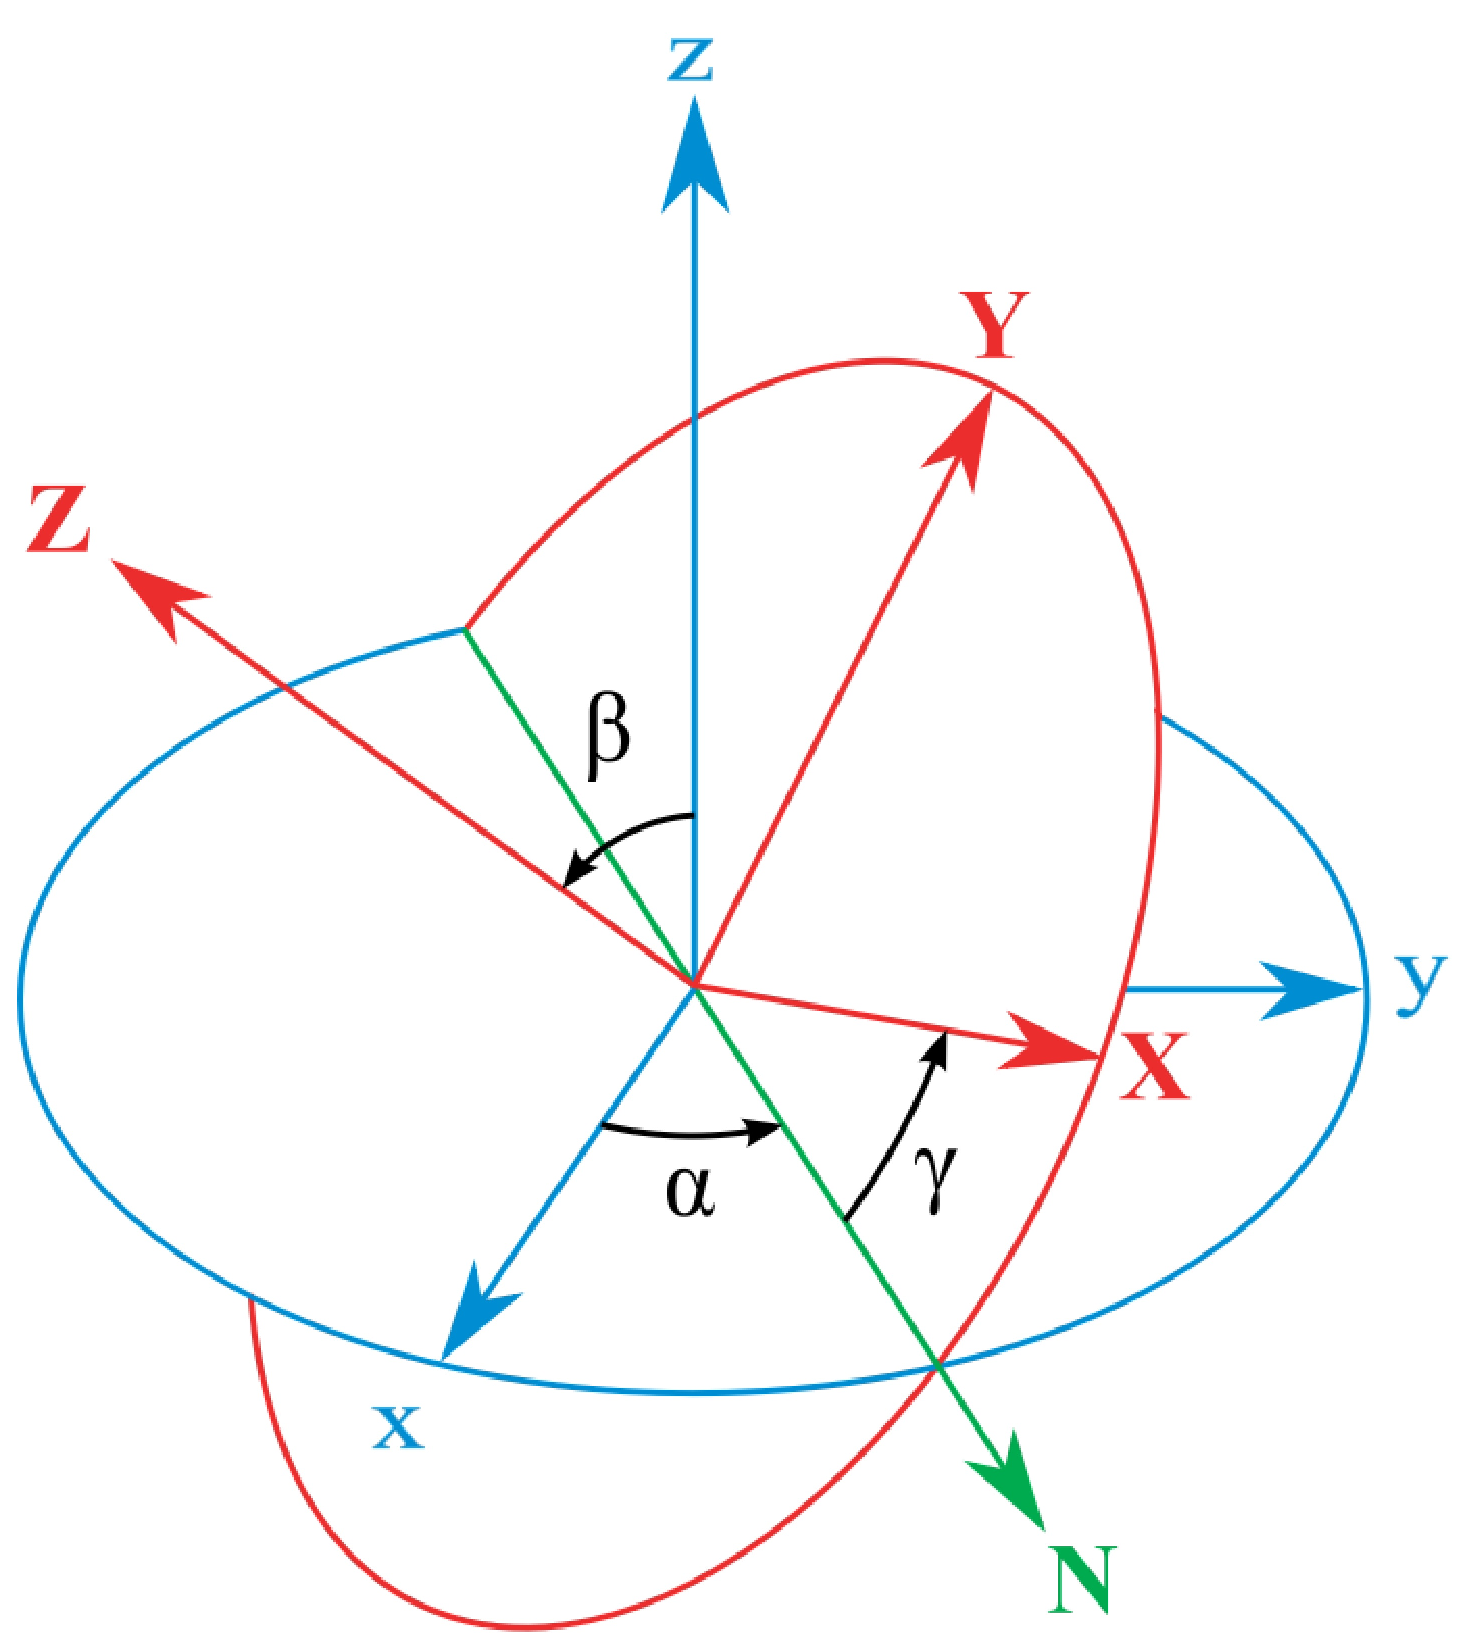
\includegraphics[scale=0.15]{Eulerangles}  \\
     \figurename{Углы Эйлера}
  \end{center}
  \begin{itemize}
  \item Угол $\alpha$ между осью $x$ и линией узлов --- угол прецессии.
  \item Угол $\beta$ между осями $z$ и $Z$ --- угол нутации.
  \item Угол $\gamma$ между осью $X$ и линией узлов --- угол собственного вращения.
\end{itemize}
 \end{frame}

\begin{frame}{Динамическое описание}
Согласно силовой модели механики равнодействующая сил приложенных к телу вызывает ускорение (второй закон Ньютона)
\begin{equation}
 \mathbf{a}=\frac{\sum\limits_{i=1}^n{\mathbf{F}_i}}{m}.
\end{equation}
\end{frame} 
 
 \begin{frame}{Геометрические примитивы} 
  \begin{center}
   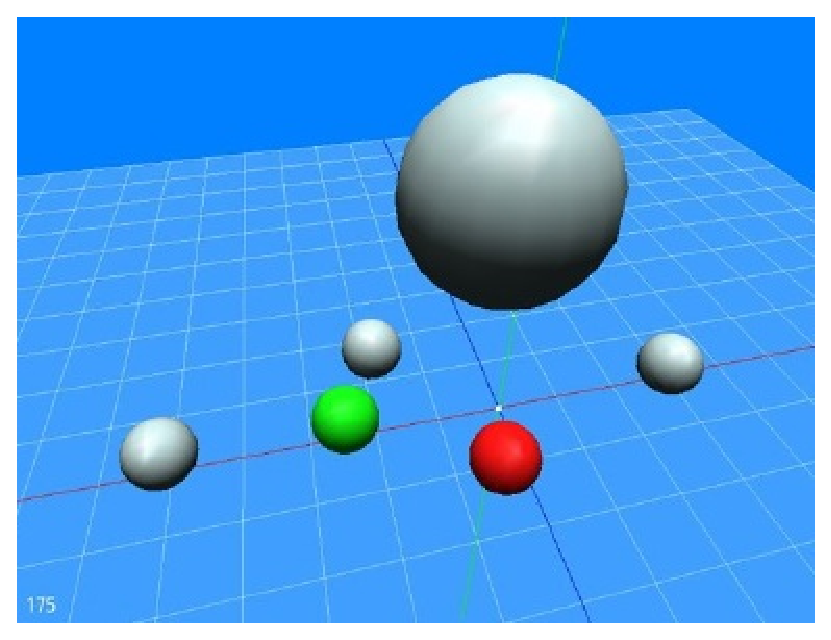
\includegraphics[scale=0.5]{Spheres}  \\
  \end{center}   
 \end{frame}
 
 
 \begin{frame}{Обнаружение столкновений}
  Модули обнаружения столкновений (\textit{collision detection}) и реагирования на столкновения (\textit{collision responce}) представляют 
  собой ключевые компоненты любого физического движка. Именно они в процессе симуляции осуществляют главную нагрузку на
  процессор, и именно от них требуется максимальная точность.
 \end{frame}
 
 \begin{frame} 
 \begin{center}
   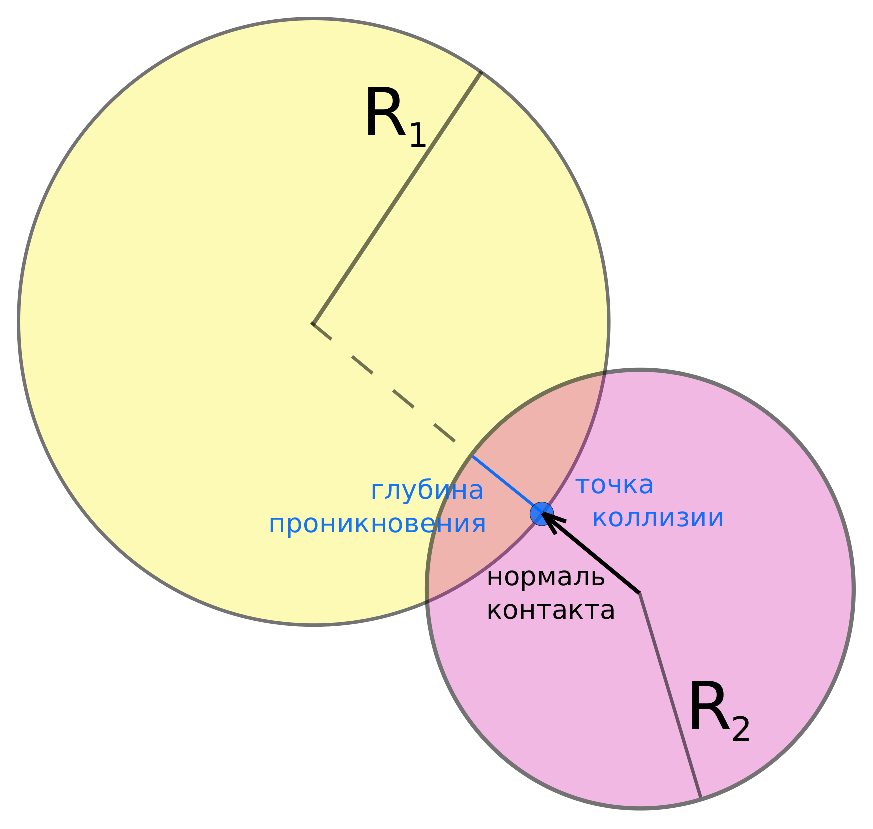
\includegraphics[scale=0.5]{SphereCollision}  \\
     \figurename{Коллизия двух сфер}
  \end{center}   
 \end{frame}

 \begin{frame}
 \begin{equation}
  \mathbf{v_{rel}} = \mathbf{v_1} - \mathbf{v_2}
  \end{equation}
 
  Если тело вращается вокруг центра масс $\mathbf{x}$  с угловой скоростью $\mathbf{\omega}$,
  то скорость его точки $\mathbf{p}$ можно выразить как
  \begin{equation}
  \mathbf{v_p} = (\mathbf{p} - \mathbf{x}) \times \mathbf{\omega} 
  \end{equation}
  
  Таким образом ограниченной степени свободы с учетом угловой скорости принимает вид:
  \begin{equation}
  \mathbf{v_{rel}} = \mathbf{v_1} + (\mathbf{p} - \mathbf{x_1}) \times \mathbf{\omega_{1}} -  \mathbf{v_2} - (\mathbf{p} - \mathbf{x_2}) \times \mathbf{\omega_{2}}
  \end{equation}
  
    Проекция относительной скорости $\mathbf{v_{rel}}$ на нормаль контакта $\mathbf{n}$ определяется скалярным произведением:
    \begin{equation}
    v_{proj} = \mathbf{v_{rel}} \mathbf{n}
    \end{equation}
    
    Потребуем: 
    \begin{equation}
    v_{proj} = 0
    \end{equation}
  \end{frame}
   
  \begin{frame}
  Если в случае с абсолютно неупругим соударением стояло условие $\mathbf{v_{proj}}$ = 0, то изменив условие следующим образом:

  \begin{equation}
  \mathbf{v_{proj}} = -bounce {v_{init}}
  \end{equation}
  
  где $v_{init}$ --- величина, равная:

  \begin{equation}
    v_{init}  = \mathbf{n_1}\mathbf{v_1} + \mathbf{w_1}\mathbf{\omega_{1}}
    + \mathbf{n_2}\mathbf{v_2} + \mathbf{w_2}\mathbf{\omega_{2}}
  \end{equation}
  
 \end{frame}
 
 \section{Заключение}
  \begin{frame}{Результаты}
  \begin{itemize}
    \item реализована объемная и гибкая библиотека математики,
    \item реализован первый геометрический примитив --- шар,
    \item используется метод Эйлера для численного решения дифференциальных уравнений,
    \item реализована гибкая физическая библиотека 
  \end{itemize}
 \end{frame} 
 
 
 
\end{document}
